\begin{figure}
  \centering
  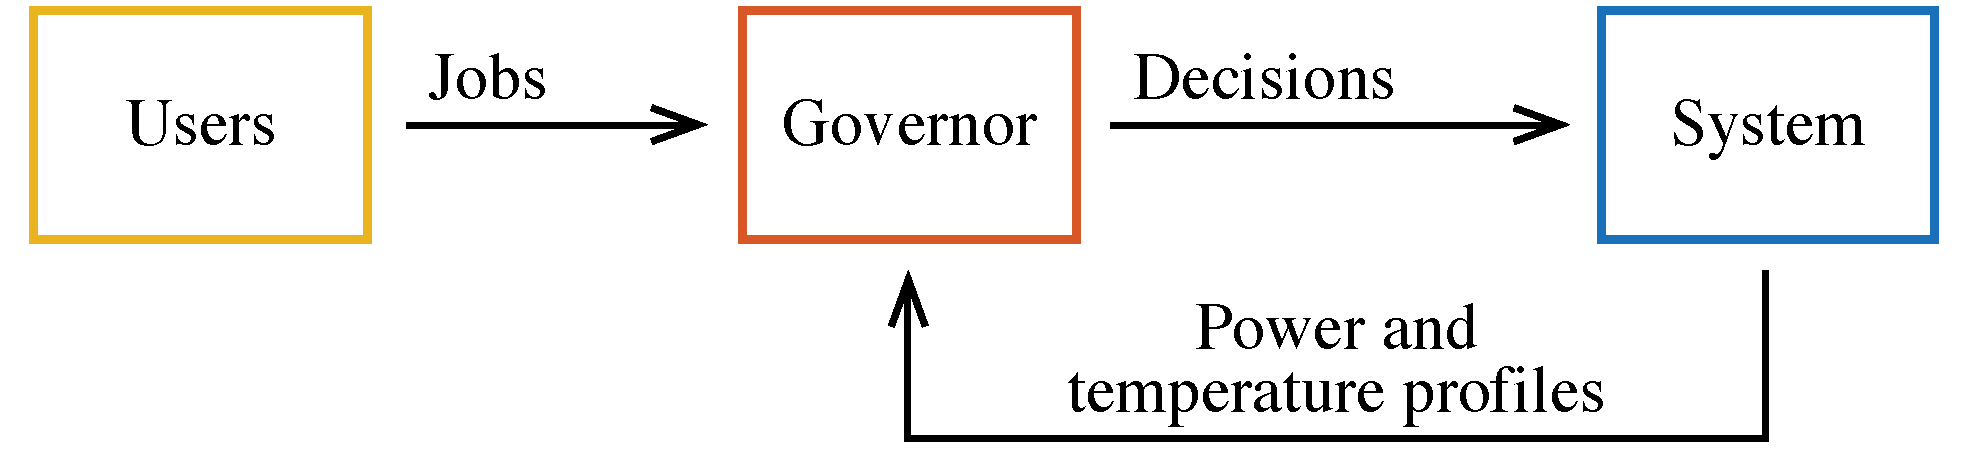
\includegraphics[width=1.0\columnwidth]{include/assets/figures/usage.pdf}
  \caption{A usage example with a feedback loop.}
  \flab{usage}
\end{figure}

Our vision of the primary usage of the proposed methodology was emphasized
throughout Sec.~\ref{sec:introduction}--\ref{sec:problem-formulation}. Having
presented the methodology and toolchain in \sref{methodology} and
\sref{toolchain}, respectively, we would like to recapitulate and give some
additional intuition. In this section, we shall look at the big picture of the
Streamer module in \fref{methodology} and the Streamer tool in \fref{streamer}.

As noted in \sref{composition} and \sref{streamer}, a scheduling or, more
generally, management policy is assumed by the data-synthesis stage of our
methodology. Conceiving and developing such a policy based on learning from the
data available on the chip is the main application of the work presented in this
paper.

From the above perspective, the methodology can be viewed as a provider of a
highly responsive development environment around the policy, which is very
unlike the prohibitively slow one depicted in \fref{development}.
Figure~\ref{fig:usage} illustrates this standpoint, in which the policy
corresponds to the module labeled ``Governor.'' The Governor module is, in a
sense, foreign to us whereas the other two modules, Users and System, are in our
jurisdiction. More concretely, the generation of a stream of jobs is an
imitation of a user behavior, which we try to replicate as realistically as
possible by using reference data. On the other hand, the synthesis of power and
temperature profiles is an imitation of the response of the underlying
electronic system to user requests and the actions taken by the governor.

One prominent usage scenario is that the management policy learns from on-chip
data and perfects itself accordingly, which is emphasized in \fref{usage} by a
feedback from the System module to the Governor module. In real life, this
feedback is readings of various hardware performance counters and sensors.

There is another scenario that we would like to mention separately, and it is a
special case of the one described above. Assure now that there is no feedback
from System to Governor in \fref{usage}. In this case, the pipeline serves the
sole purpose of generating data. These data can be stored and used for
developing techniques for the prediction of power and temperature in an abstract
setting, that is, without any specific or, perhaps, with many diverse
applications in mind.
